\section{Skinning}

{ %öffnende Klammer für hintergrundbild lokal
	\usebackgroundtemplate{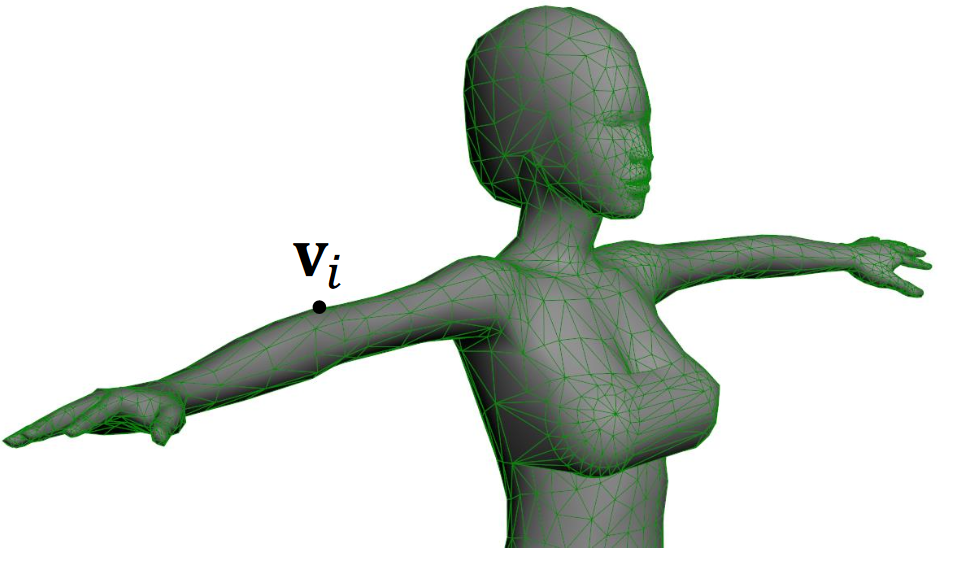
\includegraphics[width=\paperwidth,height=\paperheight]{01_Skinning/Pictures/SkinningIntro.PNG}}
	\begin{frame}{
			\begin{figure}
				\colorbox{black!10}{\Huge{Was ist Skinning?}}
			\end{figure}
		}
		\blfootnote{\colorbox{black!10}{Bildquelle: \cite{skinningcourse:2014}}}
		
		\pdfnote{Frage an alle: Was soll jetzt mit dem geriggten Modell passieren}
		\pdfnote{Frage an alle: Welcher Ansatz wäre hier der Intuitive}

		
	\end{frame}
} %schließende klammer für hintergrundbild lokal

{

	\begin{frame}{
						\begin{figure}
							\colorbox{black!10}{\Huge{Transformationen}}
						\end{figure}
			}
			
			\begin{figure}
				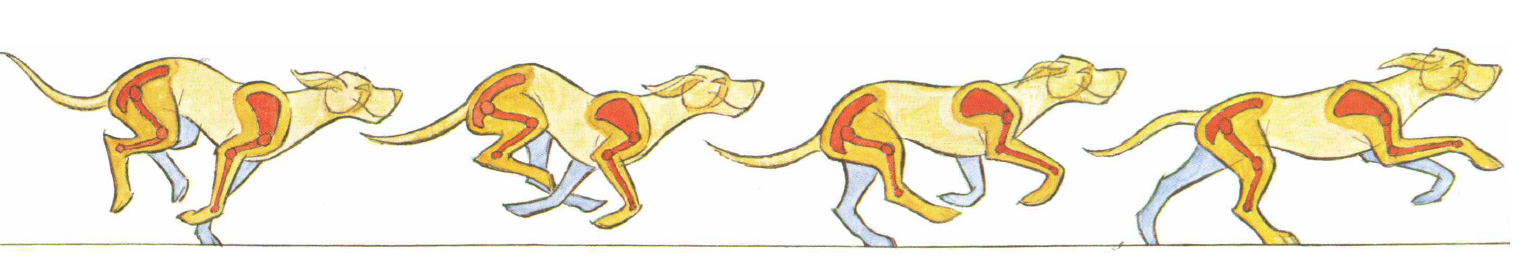
\includegraphics[width=1.0\textwidth]{01_Skinning/Pictures/Transformation.PNG}
			\end{figure}
		
		\blfootnote{\colorbox{black!10}{Bildquelle: \cite{skinningcourse:2014}}}
		
		\pdfnote{Offene Frage: Was heisst Transformation genau, wie kann man sie darstellen, was ist besonders und wichtig daran?}
		
	\end{frame}
}

	\begin{frame}{Introduction}
		\movie[]{asd}{01_Skinning/asd.avi}
		\begin{itemize}
			\item Your introduction goes here!
			\item Use \texttt{itemize} to organize your main points.
		\end{itemize}
		
		\vskip 1cm
		
		\begin{block}{Examples}
			Some examples of commonly used commands and features are included, to help you get started.
		\end{block}
		
	\end{frame}
	\pdfnote{Whatever}
	\pdfnote{zrdz}
	\pdfnote{zrdz}
	\pdfnote{zrdz}
	\pdfnote{zrdz}
	
	
	\subsection{Tables and Figures}
	
	\begin{frame}{Tables and Figures}
		
		\begin{itemize}
			\item Use \texttt{tabular} for basic tables --- see Table~\ref{tab:widgets}, for example.
			\item You can upload a figure (JPEG, PNG or PDF) using the files menu. 
			\item To include it in your document, use the \texttt{includegraphics} command (see the comment below in the source code).
		\end{itemize}
		
		% Commands to include a figure:
		%\begin{figure}
		%\includegraphics[width=\textwidth]{your-figure's-file-name}
		%\caption{\label{fig:your-figure}Caption goes here.}
		%\end{figure}
		
		\begin{table}
			\centering
			\begin{tabular}{l|r}
				Item & Quantity \\\hline
				Widgets & 42 \\
				Gadgets & 13
			\end{tabular}
			\caption{\label{tab:widgets}An example table.}
		\end{table}
		
	\end{frame}
	
	\subsection{Mathematics}
	
	\begin{frame}{Readable Mathematics}
		
		Let $X_1, X_2, \ldots, X_n$ be a sequence of independent and identically distributed random variables with $\text{E}[X_i] = \mu$ and $\text{Var}[X_i] = \sigma^2 < \infty$, and let
		$$S_n = \frac{X_1 + X_2 + \cdots + X_n}{n}
		= \frac{1}{n}\sum_{i}^{n} X_i$$
		denote their mean. Then as $n$ approaches infinity, the random variables $\sqrt{n}(S_n - \mu)$ converge in distribution to a normal $\mathcal{N}(0, \sigma^2)$.
		
	\end{frame}